\chapter{Bootproces}

\section{Opstarten}

Het opstartproces van een computer begint wanneer de voeding van
de computer ingeschakeld wordt. Bij het inschakelen controleert de
voeding zijn eigen spanningsniveaus. Wanneer de spanning stabiel is
tussen aanvaardbare waarden wordt een 'Power Good' signaal
gestuurd naar het moederbord. Het duurt typisch tussen 0,1 en 0,5
seconden voor de voeding stabiele stroom kan leveren.

Een halve seconde lijkt niet veel, maar de huidige processoren
voeren in die tijd miljoenen instructies uit. Om te vermijden dat het
systeem onder deze onstabiele omstandigheden zou beginnen opstarten
blijft het moederbord de processor continu resetten zolang er geen power
good signaal ontvangen wordt. Ook wanneer de computer al in gebruik is
verhindert dit mechanisme beschadiging of onzekere resultaten door
slechte stroomtoevoer. Bij problemen met de stroomvoorziening, zoals een
abnormale spanningswijziging op het stroomnet, zal het systeem zichzelf
herstarten omdat de processor weer tijdelijk het reset-signaal ontvangt
wanneer het power good signaal vanuit de voeding wegvalt.

Wanneer het reset-signaal wegvalt kan de processor beginnen
werken, maar welke code moet er uitgevoerd worden? Er zijn nog geen
programma's in het werkgeheugen geladen, dus de opstartcode moet elders
gevonden worden.

\section{Basic Input/Output System (BIOS)}

Het eerste programma dat de processor uitvoert is het
\emph{Basic Input/Output System}, vaak afgekort tot
\emph{BIOS}. Het zorgt dat er communicatie mogelijk is
tussen enkele onderdelen van het computersysteem, in de eerste plaats
tussen secundaire opslagapparaten en het werkgeheugen. Zo kunnen
programma's van b.v. een harde schijf in het werkgeheugen geladen
worden, en kunnen deze programma's uitgevoerd worden. Het Basic
Input/Output System dankt zijn naam aan het feit dat het naast deze
communicatie ook zorgt voor uitvoer op het scherm, en de mogelijkheid
tot invoer via het toetsenbord. Je kan de BIOS zien als een klein en
eenvoudig besturingssysteem.

Aangezien het net de BIOS ervoor moet zorgen dat de
opslagapparaten bruikbaar worden kan de BIOS-code niet op een dergelijk
apparaat bewaard worden. Daarom wordt deze code in een ROM-chip op het
moederbord bewaard. Tegenwoordig wordt EEPROM gebruikt zodat het toch
mogelijk is een nieuwe versie van de code op de chip te zetten. Deze
chip wordt ook vaak gewoon 'BIOS' genoemd. Merk op dat de BIOS opnieuw
een voorbeeld is van firmware.

Omdat een processor altijd de opdracht uit het werkgeheugen
inleest waarvan het adres in de bevelenteller staat, wordt de inhoud van
de BIOS-chip beschikbaar gesteld via een deel van het adresbereik van
het werkgeheugen. Hiervoor is een deel van het Upper Memory\footnote{De Upper
Memory Area is de laatste 384 kilobyte van de eerste megabyte van het
werkgeheugen.} gereserveerd: van F0000h tot FFFFFh. In sommige systemen
blijft dit deel van het werkgeheugen leeg en wordt van de ROM-chip
gelezen. Andere systemen kopi\"eren de inhoud van de chip naar dit
gedeelte van het werkgeheugen omdat RAM sneller is dat ROM. Deze
techniek wordt \emph{ROM shadowing} genoemd.

Wanneer een processor geactiveerd wordt zal hij altijd beginnen
met de instructie op adres FFFF0h\footnote{Het adres FFFF0h wordt ook vaak
genoteerd als FFFF:0000. De eerste notatie is lineair vanaf de start van het
werkgeheugen. De tweede notatie geeft aan dat we werken in een geheugensegment
dat begint op FFFF0, en dat we vanaf dat adres 0 plaatsen verder moeten gaan.}.
Dit adres ligt in het gebied dat aan de BIOS is toegekend, maar ligt achteraan.
Hier staat dan een JMP (jump) instrucie naar de eigenlijke opstartcode.

\subsection{Power-On Self Test}

De BIOS-opstartcode begint met het testen van de vitale
systeemonderdelen. Het geheel van deze tests wordt \emph{Power-On
Self Test} genoemd, of kortweg \emph{POST}.
De aanwezigheid en/of correcte werking van b.v. de processor,
werkgeheugen en toetsenbord worden getest. De feedback gebeurt d.m.v.
geluidssignalen die we beeps noemen. Wanneer alles naar behoren werkt
wordt meestal 1 korte beep weergegeven. Bij problemen kan men aan het
aantal beeps en hun duur horen wat de oorzaak is. De concrete codes
hangen af van de producent van de BIOS. Soms wordt bijkomend gebruik
gemaakt van bijkomende indicaties van problemen, zoals een digitaal
display of LEDs.
\subsection{Opstartvolgorde}

Als de POST succesvol voltooid is zal de BIOS-code beginnen met
het laden van het besturingssysteem. Dit staat typisch op een
secundair opslagapparaat. Wanneer een computersysteem meerdere van
dergelijke opslagapparaten bevat moet in de BIOS aangegeven zijn vanop
welk apparaat een besturingssysteem geladen moet worden. Het
besturingssysteem kan op een harde schijf staan, maar het zou ook op
een CD-ROM, diskette of USB-opslagapparaat. In welke volgorde op alle
aanwezige apparaten naar een besturingssysteem gezocht moet worden
staat in de zogenaamde \emph{opstartvolgorde} of
\emph{boot sequence}. Naast de opstartvolgorde kan je
mogelijk ook instellingen voor bepaalde randapparaten of een paswoord
dat de instellingen wijzigen.

Omdat deze instellingen gewijzigd moeten kunnen worden kunnen ze
niet samen met de code van de BIOS bewaard worden in een ROM-chip.
Voor de veranderlijke BIOS-instellingen is een afzonderlijke CMOS-chip
voorzien, die door een batterij onder spanning gehouden wordt wanneer
het systeem uitgeschakeld is. Zo gaan de instellingen niet verloren.
Omdat het in het begin de enige component met CMOS-technologie was
wordt de chip met de BIOS-instellingen nog vaak 'CMOS' genoemd. In
hedendaagse computersystemen worden echter ook de processoren en het
werkgeheugen m.b.v. CMOS ge\"implementeerd.

\subsection{Partities}

Als in de opstartvolgorde verwezen wordt naar een harde schijf
is de vraag weer hoe we het besturingssysteem terugvinden op zo'n
schijf. De code in de BIOS zal een sprong uitvoeren naar opstartcode
opgeslagen op de eerste sector van de schijf, de \emph{Master
Boot Record} (\emph{MBR}). Deze code wordt
vaak Initial Program Loader (IPL) genoemd. Na het uitvoeren van de
BIOS-code zal de processor dus verdergaan met deze code uit de
MBR.

Een harde schijf kan logisch ingedeeld worden in
\emph{partities}. Hierdoor kunnen we meerdere
besturingssystemen op \'e\'en schijf bewaren, of kunnen we op \'e\'en schijf
verschillende bestandssystemen gebruiken (zie verder).

In de \emph{partitietabel} wordt het begin- en
eindpunt en het type van iedere partitie opgeslagen. Op het
PC-platform vind je de partitietabel in de MBR, achter de opstartcode.
De opstartcode neemt 446 bytes in beslag. Er is dan nog plaats voor 4
maal een partitiebeschrijving van 16 bytes, en een 'magic number' van
2 bytes. Dit magic number is een controlgetal, en het moet de waarde
0xAA55 bevatten, anders beschouwt de BIOS de MBR als ongeldig.

\begin{figure}
\begin{center}
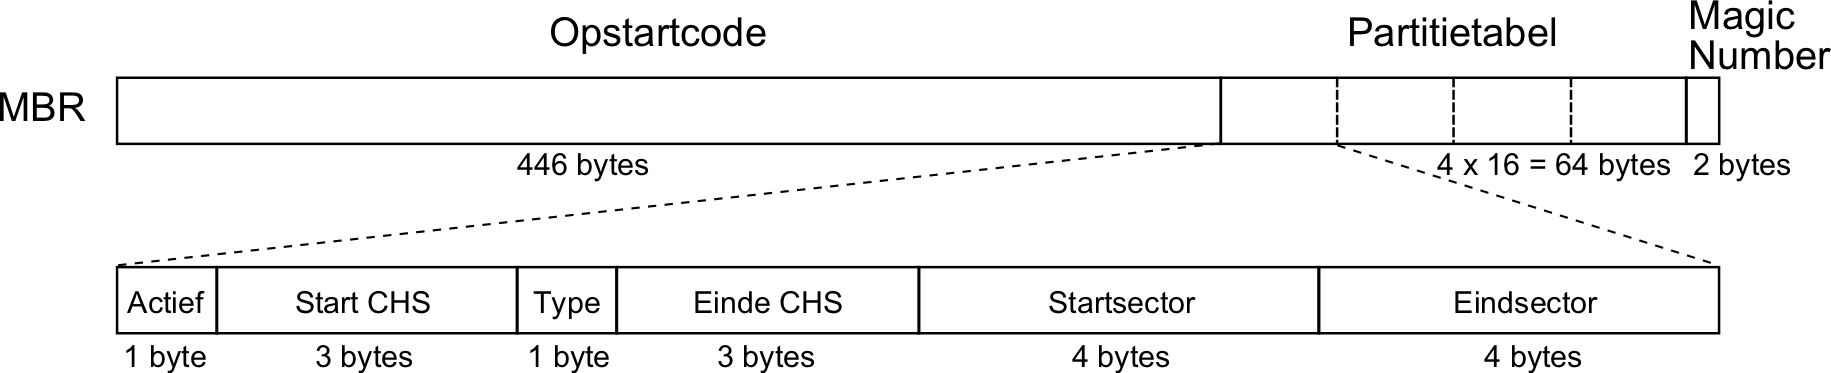
\includegraphics[width=125mm]{images/fig0206.png}
\end{center}
\caption{Master Boot Record}
\label{mbr}
\end{figure}

Elk van de 4 elementen van de partitietabel beschrijft een
partitie, en bevat de volgende velden:

\begin{description}
\item[Active] geeft aan of deze partitie opgestart moet worden
\item[Start] Cylinder / Kop / Sector adres van de eerste sector van de partitie
\item[Type] Indicatie van het gebruikte bestandssysteem op de partitie
\item[End] Cylinder / Kop / Sector adres van de laatste sector van de partitie
\item[Startsector] LBA-adres van de eerste sector van de partitie
\item[Lengte] Lengte van de partitie
\end{description}

De volledige structuur van de MBR en de partitietabel vind je in figuur
\ref{mbr}.

De partities die in de partitietabel gedefinieerd worden noemen
we \emph{primaire partities}. Doordat schijven steeds
groter werden, was 4 partities voor \'e\'en schijf niet meer genoeg. Om
meer partitities toe te laten, introduceerde men \emph{logische
partities}. Er is geen plaats om de partitietabel uit te
breiden, dus wordt een primaire partitie onderverdeeld in logische
partities. Een primaire partitie die verder onderverdeeld wordt noemen
we een '\emph{extended partitie}'. Deze oplossing is
\emph{achterwaarts compatibel}. Een ouder systeem dat
niets afweet van het bestaan van extended partities kan de gewone
primaire partities nog steeds gebruiken.

In de partitietabel geven de types 0x05 of 0x0f een extended
partitie aan. Het start-veld bevat dan het adres van de eerste sector
van de eerste logische partitie. Iedere logische partitie verwijst
naar de volgende logische partitie. Zo is er geen beperking van het
aantal logische partities door de grootte van de gebruikte tabel. Een
structuur waarin ieder element verwijst naar het volgende noemen we
een \emph{gelinkte lijst}. Als limiet voor het aantal
logische partities wordt vaak 24 opgegeven. De gelinkte lijst kan
zonder problemen langer zijn, maar aangezien MS-DOS letters vanaf 'C'
toekent aan partities kunnen er niet meer dan 24 partities
zijn\footnote{Opgelet, als je 2 primaire partities en 1 extended partitie
cre\"eert, kan je in de extended partitie natuurlijk nog maar 22 logische
partities aanmaken als je wil dat MS-DOS ze allemaal kan bereiken.}.

Een logische partitie bevat een \emph{Extended
MBR} (\emph{EMBR}), met een eigen
partitietabel. Zo'n EMBR bevat een partitietabel die de structuur van
de tabel in de MBR volgt, maar slechts twee partities beschrijft: \'e\'en
logische en een nieuwe extended partitie. Deze extended partitie bevat
ook weer zo'n tabel die \'e\'en logische en \'e\'en extended partitie
beschrijft, enz. De taak van de opstartcode in de MBR is om in de
partitietabel de actieve partitie op te sporen. De eerste sector van
deze partitie heet Partition Boot Sector (PBS), en bevat ook weer een
stuk opstartcode. De code in de MBR zal de code uit de PBS inladen en
dan door een sprong deze code uitvoeren. Het is deze code die
uiteindelijk het besturingssysteem op de partitie zal inladen en
starten. Deze code wordt in de partition boot sector geplaatst tijdens
de installatie van het besturingssysteem. In het geval van MS-DOS zal
de code in de PBS bijvoorbeeld de bestanden msdos.sys en io.sys in het
geheugen laden.
